\documentclass{article}
\usepackage[UTF8]{ctex}
\usepackage{geometry}
\usepackage{multirow}
\usepackage{natbib}
\geometry{left=3.18cm,right=3.18cm,top=2.54cm,bottom=2.54cm}
\usepackage{graphicx}
\pagestyle{plain}	
\usepackage{setspace}
\usepackage{enumerate}
\usepackage{caption2}
\usepackage{datetime} %日期
\renewcommand{\today}{\number\year 年 \number\month 月 \number\day 日}
\renewcommand{\captionlabelfont}{\small}
\renewcommand{\captionfont}{\small}
\begin{document}

\begin{figure}
    \centering
    
\includegraphics[width=8cm]{upc.png}

    \label{figupc}
\end{figure}

	\begin{center}
		\quad \\
		\quad \\
		\heiti \fontsize{45}{17} \quad \quad \quad 
		\vskip 1.5cm
		\heiti \zihao{2} 《计算科学导论》个人职业规划
	\end{center}
	\vskip 2.0cm
		
	\begin{quotation}
% 	\begin{center}
		\doublespacing
		
        \zihao{4}\par\setlength\parindent{7em}
		\quad 

		学生姓名:\underline{\qquad  黄淳 \qquad \qquad}

		学\hspace{0.61cm} 号:\underline{\qquad 1907010108\qquad}
		
		专业班级:\underline{\qquad 计科1901 \qquad  }
		
        学\hspace{0.61cm} 院:\underline{计算机科学与技术学院}
% 	\end{center}
		\vskip 1.5cm
		\centering
		\begin{table}[h]
            \centering 
            \zihao{4}
            \begin{tabular}{|c|c|c|c|c|c|c|c|c|}
            % 这里的rl 与表格对应可以看到,姓名是r,右对齐的;学号是l,左对齐的;若想居中,使用c关键字。
                \hline
                \multicolumn{5}{|c|}{分项评价} &\multicolumn{2}{c|}{整体评价}  & 总    分 & 评 阅 教 师\\
                \hline
                自我 & 环境 & 职业 & 实施 & 评估与 & 完整性 & 可行性 &\multirow{2}*{} &\multirow{2}*{}\\
                分析& 分析& 定位 & 方案 & 调整 & 20\% & 20\% & ~&~ \\\            
                10\% & 10\% & 15\% & 15\% & 10\% & &  &~ &~\\
                \cline{1-7} 
                & & & & & & & ~&~ \\
                & & & & & & & ~&~ \\
                \hline      
            \end{tabular}
        \end{table}
		\vskip 2cm
		\today
	\end{quotation}

\thispagestyle{empty}
\newpage
\setcounter{page}{1}
% 在这之前是封面,在这之后是正文
\section{自然条件}
性别:男。\par
年龄:19。\par
身体条件良好,体质正常。\par
健康状况良好,无重大遗传病或其他慢性疾病。\par
现居山东青岛。

\subsection{性格分析}
我的性格外向,善于与人交往,善于倾听。待人接物时,我能做到热情、热心和友善。我一心向善,有追求卓越的信念和信仰。我热爱我的祖国,热爱中国共产党,生活在中国特色社会主义社会中我感到很幸福。\par
但同时,外向的性格也带来了一些负面影响。譬如思考问题不够全面,面对困难不够沉稳等。

\subsection{教育与学习经历}
我毕业于一所山东省省属重点高中,在高中时代,学校提倡素质教育,因材施教。我因此得以接触到与目前所学专业相关的信息学竞赛。高中时代的经历为我适应大学生活以及在大学阶段的学习打下了坚实的基础。\par
目前我就读于全国知名的211工程大学——中国石油大学(华东)。惟真惟实的校训、勤奋、严谨、求实、创新的校风对我产生了巨大的影响。我相信,在石大读书的四年,我一定能收获满满。\par
此外,我加入了学校的ACM俱乐部,我相信这段经历一定能让我成长、提升。

\subsection{工作与社会阅历}
在学校、老师和家人的帮助下,我参加了若干次研究性学习,在社区中帮助打扫卫生,还曾经在一家涉外电商公司做过营销与英语培训的助教。这些社会与工作经历使我受益良多。

\subsection{知识、技能与经验}
目前我的计算机相关知识学习还局限在理论方面,现在的我已经掌握了部分基础算法与数据结构。我的大部分算法代码使用的面向过程的程序设计思路,部分数据结构(包括但不限于二叉搜索树及其多种平衡变种)实现了面向对象设计,并且有一定程度的抽象与封装。\par
近期在学习Python的使用,计划藉由Python深入学习面向对象的程序设计。

\subsection{兴趣爱好与特长}
我热爱数学、热爱计算机、热爱算法、数据结构与程序设计。我热爱在理论与抽象的理论体系下构建属于自己的小世界。\par
此外,我对艺术也充满了兴趣。我喜欢文学,虽然升入大学后时间很紧,我仍然保持着欣赏文学艺术与音乐艺术的习惯。我尤其喜欢余华先生的文学作品,平淡而又意味深长。语言精简、凝练。

\section{环境分析}

\subsection{社会环境分析}
现如今我们所面临的大环境十分优秀,中国社会安定,政治稳定,法制建设不断完善,文化繁荣自由,尖端技术、高新技术突飞猛进。经济发展迅速,加入WTO后,与全球一体化接轨,在全球经济一体化环境中的扮演重要角色,有大批的外国企业进入中国市场,中国的企业也将走出国门。\par
习近平总书记指出,“当前中国处于近代以来最好的发展时期,世界处于百年未有之大变局,两者同步交织、相互激荡”。无论是发展还是变局,都离不开高新技术——信息、网络、计算机、人工智能。而高新技术的发展,更离不开相关人才。目前国内的高新技术产业还是一片蓝海,而随着变局激荡、精力发展,这片蓝海一定会越来越大。

\subsection{家庭环境分析}
我有一个幸福的家庭,家庭和谐和睦,亲人和谐友善。有着家中长辈们的关怀、关爱与支持,特别是父母对我的期望、祝福以及不遗余力的支持;父母将巨大的精力与金钱投资到了我的身上,并且给我无私不求回报的爱。我生活在一个幸福的家庭中,我觉得我是个幸运的人,也是个幸福的人。\par
而我的父母长辈们的观念并不传统保守,他们支持我外出闯荡,支持我努力追求自己人生的价值与梦想,支持我在世界的任何一个角落为祖国,为中国人民,为社会主义世界流汗流血、奋斗。

\subsection{职业环境分析}
从国内外市场总体发展情况来看,随着中国逐渐成为全球IT企业关注的重心,在国内外IT市场上的话语权越来越大,中国IT业市场的竞争日趋激烈、IT企业对人才的要求不但越来越高,而且要求瞬息万变。中国不但已经成为全球重要的IT制造中心,同时也逐渐步入全球IT研发中心的角色。良好的国内经济环境及全球化大环境使中国IT行业市场保持平稳的增长,蓬勃发展的中国软件与IT服务市场吸引了众多海内外投资者与创业者。\par
展望未来,中国国民经济将继续保持稳步的增长,中国行业和企业信息化建设进一步深化,消费者消费水平逐步提高,中国IT行业市场具有良好的发展前景。

\subsection{地域与人际环境分析}
杭州作为长江三角洲地区的重要城市,在新中国历史发展进程中起到了举足轻重的作用。不仅是改革开放的试验田,也是习近平总书记曾经工作、奋斗过的地方。\par
直到今天,浙江、杭州的多项政策,在全国范围来看,仍然具有超前性与前瞻性。\par
杭州气候宜人,有西湖、西溪等湿地及湖泊,多丘陵,植被覆盖率高。但是良好的生态环境并没有影响杭州的发展。得益于党的领导,杭州的发展真正实现了人与自然和谐相处,实现了绿水青山就是金山银山。

\begin{figure}[h!]
\centering
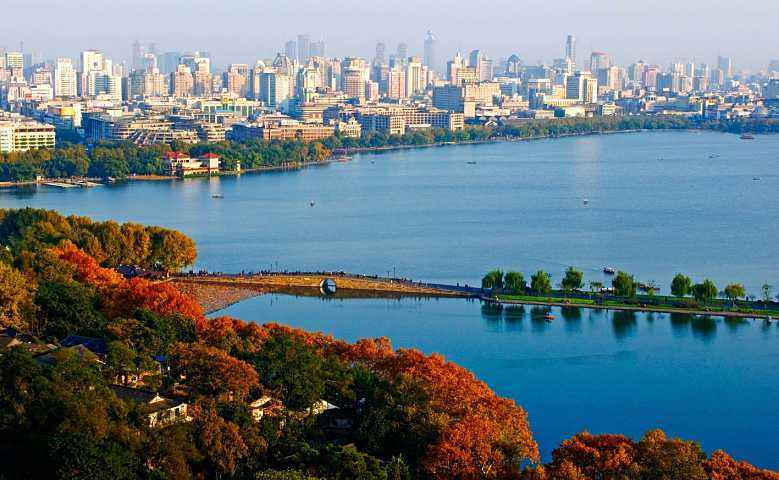
\includegraphics[scale=0.55]{timg}
\caption{杭州}
\label{fig:timg}
\end{figure}



\section{职业定位}
\subsection{行业领域定位与理由}
目前诸多企业对算法岗位需求巨大。\par
对企业而言,自主知识产权是立身之本,只有像华为这样有自主研发能力,有大量自主知识产权的企业才能勇攀高峰,在诸多浪潮中屹立不倒。\par
而自主知识产权的核心之一就是优秀的算法与架构设计。
\subsection{职业岗位起点定位与理由}
我希望在有社会责任感,符合社会主义核心价值观的国际知名企业中成为一名算法工程师。\par
于我本人而言,我不满足于懂得表象,更喜欢深入研究,喜欢钻研事物的本质。在数学、算法和数据结构的学习中,我也十分重视证明、重视知其然且知其所以然。\par
并且,对于IT产业、网络产业以及其他新兴信息技术相关产业而言,拥有自主知识产权的技术是企业发展的重中之重。在过去的几年里,联想向美国人示弱、示好、求饶,中兴被美国的政策击溃而华为却在贸易战的浪潮中屹立不倒,成为美国的眼中钉、肉中刺,成为中国民族企业的希望、成为国之利器,恰好能说明这一点。而算法正是信息技术的核心。\par
我希望能在像华为、阿里这样有社会责任感、积极传播社会主义核心价值观的优秀民族企业、国际知名企业中,为中华民族伟大复兴的中国梦奉献我的奋斗与力量。
\subsection{职业目标与可行性分析}
\begin{enumerate}[(1)]
	\item {
		短期目标(大学4年)
		\begin{itemize}
			\item {认真完成学校为本专业指定的发展计划。}
			\item {在学校的学习中取得优秀的成绩,掌握发展计划中的各项要求。}
			\item {积极参与算法竞赛的训练,获得充足的算法竞赛相关知识。}
			\item {在国内外算法竞赛中证明自己的能力。}
			\item {寻找机会深入企业参与实习。}
		\end{itemize}
	}
	\item {
		中长期目标(5-10年)
		\begin{itemize}
			\item {入职国际知名优秀企业。}
			\item {尽快学习并熟练掌握自己的工作内容。}
			\item {奋斗拼搏,在工作中实践创新。}
			\item {进入所在企业的部门研发核心。}
			\item {成为算法研究员。}
		\end{itemize}
	}
\end{enumerate}
短期目标中的前两条,是一名大学生必须有的目标,是当代大学生的分内工作。习近平总书记曾在多个场合向全国人民发出奋斗动员令:“幸福都是奋斗出来的”、“奋斗本身就是一种幸福”。而作为一名大学生,我也不例外,理应趁着最好的青春年华,拼搏奋斗提升自己。\par
现如今,在课余时间,我积极参与算法竞赛的训练。无论是校内ACM俱乐部的例行训练,还是国内外知名网站,如杭州电子科技大学在线评测网站、牛客网和Codeforces举办的网上训练比赛,都使我受益匪浅。有志者事竟成,我有理由相信,锲而不舍的训练一定能换来一个更加优秀的自己。\par
而对于长期目标而言,其成功与否并非如今的我可以妄加判断。我只知道,每一个长期目标的实现,都需要短期目标的完成作为基石。我相信,拼尽全力奋斗大学四年,奋斗和拼搏的结果一定不会让我失望。


\section{实施方案}
\begin{enumerate}[1、]
	\item {努力学习,在学校规定的学习科目中取得优秀成绩。}
	\item {立足于自己有竞赛基础、算法基础、较为丰富的程序设计经验,积极参与各种竞赛与项目,全方位提升自己的相关能力。}
	\item {培养攻坚克难的习惯与信念,勇于挑战未知领域与未知知识,通过攻坚克难让自己取得全局思考的能力与沉稳且有条理的心态。}
	\item {积极与优秀的老师交流,与成功的学长交流,听取老师的建议和引导,在学长学姐成功的经历中获取经验。}
	\item {孝敬父母,拿出足够的时间和父母沟通交流。}
	\item {若干年后,组建家庭时,寻求可以和我共同承担压力,同甘共苦共患难的配偶。}
	\item {继续培养自己对文学和艺术的热爱,藉由文学艺术释放工作压力,保证身心健康。}
\end{enumerate}


\section{评估与调整}

\subsection{评估时间}
每学期评估一次

\subsection{评估内容}
可以从成果目标、经济目标、能力目标、职务目标等方面总结,确定哪些目标已按预期实现,哪些目标商未达到,对已实现的成果总结经验,对未完成的目标分析原因。\par
首先,分析自己的学业成绩以及一学期内自己对公共基础课、专业基础课、专业课的学习态度、学习状态及学习成果,包括个人的学习收获。\par
其次,分析自己在算法竞赛训练中的提升与不足,以及在算法竞赛中取得的成绩。\par
第三,分析自己在本学期内参加的各项工程实践活动所带来的收获与感悟。\par
在如上的评估中总结自己一学期内的收获与不足,从宏观和大局观上分析,及时调整自己的状态与目标。

\subsection{调整原则}
首先,根据自身对所制定目标的适应性,目标与自身的匹配性进行调整。\par
其次,环境瞬息万变,应关注时事,关心形式变化,及时调整目标。\par
最后,若所制定目标在操作上可行性较差,应及时调整。



\end{document}
